
\hypertarget{cv:registrarModulo}{\section{Registrar Módulo}} \label{sec:registrarModulo}

	Esta funcionalidad le permitirá registrar un módulo dentro del proyecto que se esta operando, una vez registrado podrá empezar a gestionar los casos de uso, así como todas las acciones que le competen dentro del proyecto. 

		\subsection{Procedimiento}

			%Pasos de procedimiento
			\begin{enumerate}
	
			\item Oprima el botón \IURegistrar{} de la pantalla \ref{fig:GestionarModulos} ''Gestionar Módulos''.
			
			\item Se mostrará la pantalla \ref{fig:registrarModulo} ''Registrar Módulo''.

			%Pantalla
			\begin{figure}[htbp!]
				\begin{center}
					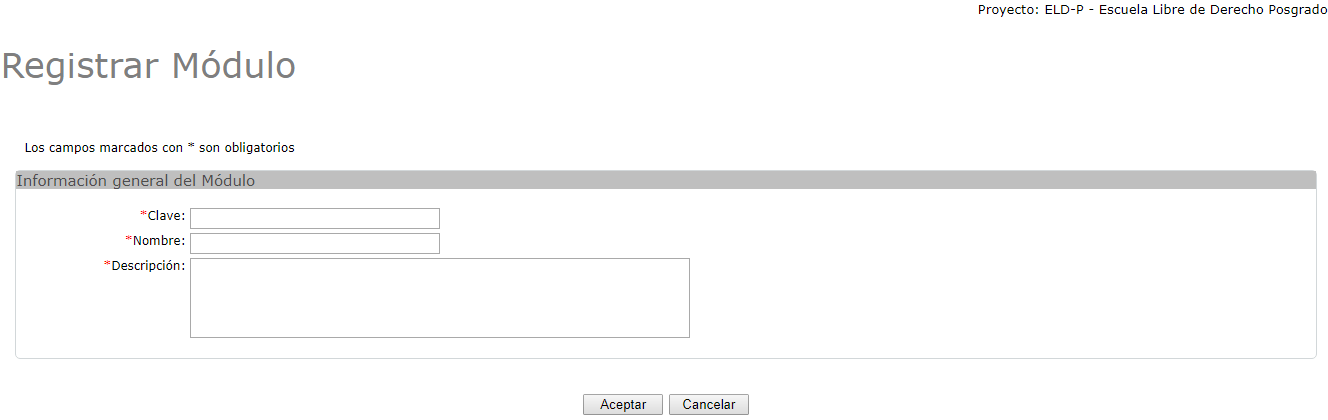
\includegraphics[scale=0.5]{roles/lider/modulos/pantallas/IU5-1registrarModulo}
					\caption{Registrar Módulo}
					\label{fig:registrarModulo}
				\end{center}
			\end{figure}
		
			\item Ingrese la clave con el cual se identificará el módulo, un nombre y una pequeña descripción del mismo indicando que parte de la funcionalidad del sistema se esta tratando dentro del módulo.
			
			\item Oprima el botón \IUAceptar.
			
			\item Se mostrará el mensaje \ref{fig:moduloRegistrado} en la pantalla \ref{fig:GestionarModulos} ''Gestionar Módulos''.
			
			\begin{figure}[htbp!]
				\begin{center}
					
\includegraphics[scale=0.6]{roles/lider/modulos/pantallas/IU5-1MSG1}
					\caption{MSG: Módulo Registrado}
					\label{fig:moduloRegistrado}
				\end{center}
			\end{figure}
			\end{enumerate}